% Provenance (never printed): see sources/outline_sources.md (Year 3:
% Glen's flow law; mass balance; ice sheets and ice shelves; sea ice;
% permafrost; the cryosphere's contribution to sea level).
% Brief: sources/book5/BRIEFS.md, ch. 24. Curves from figdata/bachelor-3/
% ice_flow.py (Glen slab, the plastic profile against the ETOPO1 Greenland
% transect, the Arkel ice cap) and sea_ice.py (NSIDC March and September
% extents, Stefan's law). Exercise and problem values in the Book 5 scratch
% calculator calc/ch24.py. The Arkel ice cap and the glaciers of the
% exercises are invented.
\chapter{Glasiologi}\label{ch:b3:glaciology}

Lintasi Greenland dari barat ke timur sepanjang paralel \ang{72.5}~LU. Es
mulai beberapa puluh kilometer ke arah daratan, menanjak curam, lalu makin
landai hingga mencapai puncak yang luas setinggi \qty{3229}{m}, lalu turun
kembali ke pegunungan di pantai timur. Jika diplot, permukaannya hampir
menyerupai parabola yang berbaring miring, dengan puncaknya di tepi. Bab ini
menunjukkan dari mana bentuk itu berasal: dari suatu bahan yang merayap
semakin cepat ketika ditekan semakin kuat, sehingga hampir seolah tidak
mampu menahan tegangan lebih dari nilai tertentu. Setelah itu, bab ini
mengikuti es dari salju yang memberinya makan hingga laut yang menerimanya.
% ledger: data:b5-etopo-greenland

\begin{recall}
Gletser, lembaran es, paparan es, gunung es, es laut, permafrost, dan zaman es
sudah dibahas dalam buku-buku sekolah. \omterm{def:b3:deformation-mechanisms:flow-law}{Hukum aliran} dan \omterm{def:b3:deformation-mechanisms:creep}{rayapan dislokasi} dibahas
pada Bab~\ref{ch:b3:deformation-mechanisms}; \omterm{def:b3:gravity-geodesy:satgrav}{gravimetri satelit} dan
neraca massa lembaran es yang diukurnya dibahas pada Bab~\ref{ch:b3:gravity-geodesy};
inti es dan isotop oksigennya dibahas pada Bab~\ref{ch:b3:stable-isotopes}.
Anggaran permukaan laut, umpan balik es--albedo, dan kenaikan permukaan laut
termosterik dibahas pada volume Tahun~2, dalam bab tentang perubahan iklim
akibat aktivitas manusia. Kalor laten dan konduksi kalor dibahas dalam buku fisika.
\end{recall}

\section{Es sebagai bahan}\label{sec:b3:glaciology:material}

Es gletser adalah batuan, yakni massa kristal es yang saling mengunci, dan es
itu berubah bentuk mendekati titik lelehnya. Di bawah tegangan, es merayap
melalui gerakan \omterm{def:b3:deformation-mechanisms:dislocation}{dislokasi} di dalam kristalnya, seperti batuan pada
Bab~\ref{ch:b3:deformation-mechanisms}, dan \omterm{def:b3:deformation-mechanisms:flow-law}{hukum alirannya} memiliki bentuk
yang sama: pangkat tegangan dikali faktor Arrhenius.

\begin{theorem}[Hukum aliran Glen]\label{thm:b3:glaciology:glen}
Pada es gletser isotropik, tensor laju regangan sebanding dengan
tegangan deviatorik,
\[
\dot\varepsilon_{ij} = A(T)\,\tau_e^{\,n-1}\,\tau'_{ij}, \qquad
\tau_e^2 = \tfrac12\,\tau'_{ij}\tau'_{ij},
\]
dengan $n = 3$ dan \omterm{def:b3:glaciology:glen}{faktor laju} $A(T)$ yang membesar seiring suhu. Pada
geser sederhana, dengan $\tau_{xz}$ sebagai satu-satunya tegangan deviatorik yang tidak nol,
$\dot\varepsilon_{xz} = A\tau_{xz}^{\,n}$.
\end{theorem}
\index{hukum aliran Glen}

\begin{proof}
Hukum ini sendiri bersifat empiris: fungsi pangkat yang dicocokkan dengan eksperimen rayapan dan
deformasi gletser; koefisien dan eksponennya dicocokkan
bersama. Pada geser sederhana $\tau'_{xz} = \tau'_{zx} = \tau_{xz}$ dan
komponen lainnya nol, sehingga $\tau_e^2 = \tfrac12(\tau_{xz}^2 +
\tau_{zx}^2) = \tau_{xz}^2$, dan $\dot\varepsilon_{xz} = A\tau_{xz}^{\,n-1}
\tau_{xz}$.
\end{proof}
% ledger: pism:rheology

Dengan $n = 3$, es merupakan fluida yang sangat tak-linear: menggandakan
tegangan membuatnya berubah bentuk delapan kali lebih cepat. Viskositas efektifnya, $1/(2A\tau_e^{\,2})$,
bukan sifat es semata, melainkan turun seiring naiknya tegangan.

\begin{definition}[Faktor laju (es)]\label{def:b3:glaciology:glen}
Dalam hukum Glen, \emph{faktor laju}\index{faktor laju (es)} $A(T)$, yang juga
disebut kelunakan es, ditulis $A = A_0\exp(-Q/RT)$, dengan
energi aktivasi $Q$. Suatu kecocokan yang luas dipakai (Paterson dan Budd) mengambil $A_0 =
\qty{3.61e-13}{s^{-1}.Pa^{-3}}$ dan $Q = \qty{60}{kJ/mol}$ di bawah
\qty{-10}{\celsius}, serta $A_0 = \qty{1.73e3}{s^{-1}.Pa^{-3}}$ dan $Q =
\qty{139}{kJ/mol}$ di atasnya, yaitu lebih dekat ke titik leleh, tempat es
melunak lebih cepat terhadap suhu.
\end{definition}
% ledger: pism:rheology, codata:R

\begin{center}
\begin{tabular}{lccc}
\hline
suhu & \qty{-25}{\celsius} & \qty{-10}{\celsius} & \qty{0}{\celsius}\\
$A$ (\unit{Pa^{-3}.yr^{-1}}) & \num{2.7e-18} & \num{1.4e-17} & \num{1.4e-16}\\
\hline
\end{tabular}
\end{center}

Es pada titik lelehnya mengalir sekitar lima puluh kali lebih cepat dibandingkan
pada \qty{-25}{\celsius} di bawah tegangan yang sama. Tegangan di dalam gletser
berorde satu bar, \qty{e5}{Pa}.
% ledger: pism:rheology

Gletser bergerak dengan dua cara. Es di dalamnya berubah bentuk dengan rayapan, di mana saja; dan
di tempat dasarnya berada pada titik leleh, es juga dapat meluncur.

\begin{definition}[Gelincir basal]\label{def:b3:glaciology:sliding}
Yang disebut \emph{gelincir basal}\index{gelincir basal} adalah gerakan gletser di atas
dasarnya, pada lapisan air tipis atau lapisan sedimen lunak yang basah. Gelincir ini
memerlukan dasar pada titik leleh; gletser yang membeku pada dasarnya hanya bergerak
melalui rayapan esnya.
\end{definition}
% ledger: nsidc:glacier-flow

\section{Aliran gletser}\label{sec:b3:glaciology:flow}

\begin{theorem}[Aliran lempengan dengan sisi sejajar]\label{thm:b3:glaciology:slab}
Suatu lempengan es berketebalan $H$ dan massa jenis $\rho$ terletak di atas dasar dengan kemiringan
$\alpha$ dan mengalir ke bawahnya dengan geser sederhana, meluncur dengan kecepatan $u_b$. Pada
ketinggian $z$ di atas dasar, tegangan gesernya adalah $\tau = \rho g(H - z)\sin\alpha$,
kecepatannya
\[
u(z) = u_b + \frac{2A}{n + 1}(\rho g\sin\alpha)^n\left[H^{n+1} - (H -
z)^{n+1}\right],
\]
dan fluks per satuan lebar $q = u_bH + \dfrac{2A}{n + 2}(\rho
g\sin\alpha)^nH^{n+2}$. Tegangan geser dasarnya adalah $\tau_b = \rho gH\sin\alpha$.
\end{theorem}

\begin{proof}
Es di atas ketinggian $z$ memiliki berat $\rho g(H - z)$ per satuan luas; komponennya
sepanjang lereng, $\rho g(H - z)\sin\alpha$, diseimbangkan oleh
tegangan geser pada dasarnya, karena permukaan bebas dari tegangan. Menurut hukum Glen,
$\mathrm du/\mathrm dz = 2\dot\varepsilon_{xz} = 2A\tau^n$; dengan mengintegralkan dari
dasar, tempat $u = u_b$, diperoleh $u(z)$, dan dengan mengintegralkan $u$ dari 0 ke $H$
diperoleh $q$.
\end{proof}

Kecepatan berubah sedikit di bagian atas lempengan dan cepat di dekat
dasar, tempat tegangannya paling besar: untuk $n = 3$ geser terkonsentrasi di
lapisan paling bawah. Kecepatan permukaan tumbuh sebanding dengan $H^{n+1} = H^4$ dan dengan
pangkat tiga kemiringan: gletser dua kali lebih tebal mengalir enam belas kali lebih cepat.

\begin{definition}[Pendekatan es dangkal]\label{def:b3:glaciology:sia}
\emph{Pendekatan es dangkal}\index{pendekatan es dangkal} memperlakukan
lembaran es yang ketebalannya kecil dibandingkan lebarnya sebagai lempengan
dengan sisi sejajar secara lokal: di setiap tempat es berdeformasi oleh geser sederhana di bawah
\emph{tegangan pendorong} $\tau_d = \rho gH|\nabla s|$, dengan $s$ adalah
ketinggian permukaan, dan fluks mengikuti rumus lempengan dengan
ketebalan lokal dan kemiringan permukaan.
\end{definition}

Dalam \omterm{def:b3:glaciology:sia}{pendekatan es dangkal}, tegangan dasar ditentukan oleh bentuk
es. Karena laju regangan naik sebagai pangkat tiga tegangan, kenaikan tegangan yang
sedikit saja menghasilkan kenaikan aliran yang besar, yang menipiskan es
dan menurunkan tegangan lagi: tegangan tetap berada dalam rentang yang sempit,
berapa pun ukuran massa es. Jika ini dibawa sampai batasnya, sebuah bahan yang
sama sekali tidak berdeformasi di bawah tegangan luluh $\tau_0$ dan berdeformasi tanpa
batas di atasnya, dan bentuknya mengikuti.

\begin{proposition}[Profil lembaran es plastis]\label{prop:b3:glaciology:nye}
Lembaran es sepenuhnya plastis dengan tegangan luluh $\tau_0$ di atas dasar
horizontal yang datar, pada jarak $x$ ke arah daratan dari tepinya, memiliki tinggi permukaan
\[
h(x) = \sqrt{\frac{2\tau_0x}{\rho g}} .
\]
\end{proposition}
\index{profil lembaran es plastis}

\begin{proof}
Di mana-mana tegangan dasar sama dengan tegangan luluh: $\rho gh\,\mathrm
dh/\mathrm dx = \tau_0$, dengan kemiringan kecil. Maka $\mathrm d(h^2)/\mathrm
dx = 2\tau_0/(\rho g)$, dan $h = 0$ di tepi.
\end{proof}

\begin{omfigure}
\begin{tikzpicture}
\begin{groupplot}[group style={group size=2 by 1, horizontal sep=1.5cm},
  height=0.4\linewidth,
  tick label style={font=\scriptsize}, label style={font=\small}, title style={font=\small}]
\nextgroupplot[width=0.38\linewidth, xlabel={$u/u_s$}, ylabel={tinggi di atas dasar, $z/H$},
  xmin=0, xmax=1.05, ymin=0, ymax=1, title={Lempengan},
  legend style={font=\scriptsize, at={(0.03,0.97)}, anchor=north west}]
% computed in figdata/bachelor-3/ice_flow.py
\addplot[omThm, thick] table[x=u3, y=zeta] {figdata/out/bachelor-3-ice_flow-slab.dat};
\addlegendentry{$n = 3$}
\addplot[omDef, thick, densely dashed] table[x=u1, y=zeta] {figdata/out/bachelor-3-ice_flow-slab.dat};
\addlegendentry{$n = 1$}
\addplot[omMeth, thick] table[x=u3b, y=zeta] {figdata/out/bachelor-3-ice_flow-slab.dat};
\addlegendentry{$n = 3$, gelincir}
\nextgroupplot[width=0.58\linewidth, xlabel={jarak dari \ang{58}BB sepanjang \ang{72.5}LU (\unit{km})},
  ylabel={ketinggian (\unit{m})}, xmin=0, xmax=1270, ymin=-500, ymax=3700,
  title={Greenland}, scaled x ticks=false, xticklabel style={/pgf/number format/1000 sep={}},
  scaled y ticks=false, yticklabel style={/pgf/number format/1000 sep={}},
  legend style={font=\scriptsize, at={(0.5,0.03)}, anchor=south}]
\addplot[black, thin] table[x=x, y=h] {figdata/out/bachelor-3-ice_flow-gl.dat};
\addlegendentry{es dan permukaan daratan}
\addplot[omThm, thick, densely dashed] table[x=x, y=h] {figdata/out/bachelor-3-ice_flow-nye-w.dat};
\addlegendentry{profil plastis}
\addplot[omThm, thick, densely dashed, forget plot] table[x=x, y=h] {figdata/out/bachelor-3-ice_flow-nye-e.dat};
\draw[black!40] (axis cs:0,0) -- (axis cs:1270,0);
\node[font=\scriptsize, omThm, align=center] at (axis cs:330,2900) {$\tau_0 = $\\ \qty{72}{kPa}};
\node[font=\scriptsize, omThm, align=center] at (axis cs:1040,2900) {$\tau_0 = $\\ \qty{108}{kPa}};
\end{groupplot}
\end{tikzpicture}

\par\smallskip{\small Kiri, kecepatan melintasi lempengan es, diskalakan dengan
kecepatan permukaan: hukum Glen ($n = 3$) memusatkan geser di dekat dasar, sedangkan
fluida linear ($n = 1$) menyebarkannya; dengan gelincir, seluruh profil
bergeser. Kanan, permukaan Greenland sepanjang \ang{72.5}LU (ETOPO1 Ice
Surface, NOAA NCEI), dan profil plastis yang dicocokkan pada kedua sisinya, untuk
ketinggian di atas \qty{1000}{m} dan dasar yang diambil pada permukaan laut. Pencocokan memerlukan
tegangan luluh \qty{72}{kPa} dan \qty{108}{kPa}, sebanding dengan orde bar pada
gletser sungguhan; profil ini meleset di tepi yang curam, tempat dasar dan pencairan
berperan.}\label{fig:b3:glaciology:flow}
\end{omfigure}
% ledger: data:b5-etopo-greenland, pism:rheology

\section{Neraca massa}\label{sec:b3:glaciology:mass-balance}

Gletser mendapat pasokan dari salju dan kehilangan es karena pencairan, penguapan, dan, bila
mencapai perairan, karena \omterm{def:b3:glaciology:grounding-line}{pelepasan bongkah es}.
% ledger: nsidc:glacier-zones

\begin{definition}[Neraca massa; zona akumulasi dan ablasi; garis kesetimbangan]\label{def:b3:glaciology:mass-balance}
Yang disebut \emph{neraca massa gletser}\index{neraca massa gletser} adalah perubahan
massa gletser selama satu tahun, biasanya dinyatakan dalam meter air
setara yang dirata-ratakan terhadap luasnya. Bagian \emph{neraca massa
permukaan}\index{neraca massa permukaan} adalah bagian yang disebabkan oleh proses di
permukaan, yaitu salju turun dikurangi pencairan, limpasan, dan sublimasi; sisanya
hilang karena \omterm{def:b3:glaciology:grounding-line}{pelepasan bongkah es} dan pencairan di dasar atau di bawah es terapung.
Yang dimaksud dengan \emph{zona akumulasi}\index{zona akumulasi} adalah bagian dari
permukaan tempat neraca massa permukaan selama setahun bernilai positif, sedangkan
\emph{zona ablasi}\index{zona ablasi} adalah bagian tempat nilainya negatif,
serta \emph{ketinggian garis kesetimbangan}\index{ketinggian garis kesetimbangan}
(ELA) adalah ketinggian garis yang memisahkan keduanya, tempat nilainya nol.
\end{definition}

\begin{omfigure}
\centering
\begin{tikzpicture}[>=stealth, font=\small, x=1cm, y=1cm]
% bed and surface of a valley glacier, long section
\fill[black!12] (0,0) -- (0,4.6) .. controls (2,3.6) and (6,1.4) .. (11,0) -- cycle;
\fill[omSea!45] (0,4.6) .. controls (2,3.6) and (6,1.4) .. (11,0)
  -- (11,0) .. controls (8,1.0) and (4,3.2) .. (0.6,5.4) -- (0,5.6) -- cycle;
\draw[thick, black!70] (0,4.6) .. controls (2,3.6) and (6,1.4) .. (11,0);
\draw[thick, omDef] (0,5.6) -- (0.6,5.4) .. controls (4,3.2) and (8,1.0) .. (11,0);
% equilibrium line
\draw[omThm, densely dashed, thick] (5.0,2.76) -- (5.0,4.6);
\node[omThm, font=\scriptsize, anchor=south] at (5.0,4.6) {garis kesetimbangan (ELA)};
% balance arrows
\foreach \x/\y in {1.2/5.02, 2.4/4.27, 3.6/3.56} {\draw[->, omDef, thick] (\x,\y+0.55) -- (\x,\y+0.05);}
\foreach \x/\y in {6.4/2.02, 7.6/1.42, 8.8/0.86} {\draw[->, omThm, thick] (\x,\y+0.02) -- (\x,\y+0.52);}
\node[omDef, font=\scriptsize, align=center] at (2.4,6.2) {zona akumulasi:\\salju yang bertambah};
\node[omThm, font=\scriptsize, align=center] at (8.6,2.5) {zona ablasi:\\es yang hilang};
% flow lines, computed inside the ice: buried in the accumulation zone, emerging in the ablation zone
\draw[->, black!60] plot[smooth] coordinates {(1.00,5.14) (1.98,4.28) (2.95,3.54) (3.93,2.93) (4.90,2.43) (5.88,2.00) (6.85,1.62) (7.83,1.24) (8.80,0.86)};
\draw[->, black!60] plot[smooth] coordinates {(2.20,4.39) (2.84,3.89) (3.48,3.43) (4.11,3.02) (4.75,2.67) (5.39,2.36) (6.03,2.08) (6.66,1.82) (7.30,1.56)};
\draw[->, black!60] plot[smooth] coordinates {(3.40,3.67) (3.74,3.44) (4.08,3.21) (4.41,3.00) (4.75,2.81) (5.09,2.63) (5.42,2.47) (5.76,2.32) (6.10,2.17)};
\node[font=\scriptsize, anchor=north east] at (10.9,-0.1) {moncong};
\node[font=\scriptsize] at (3.0,1.4) {batuan dasar};
\end{tikzpicture}

\par\smallskip{\small Penampang memanjang skematis gletser lembah dalam
keseimbangan. Di atas garis kesetimbangan, salju setiap tahun terkubur dan
terbawa ke dalam gletser; di bawahnya, permukaan kehilangan es setiap tahun dan
diperbarui oleh es yang naik dari kedalaman. Garis aliran (abu-abu) miring di
\omterm{def:b3:glaciology:mass-balance}{zona akumulasi} dan naik di \omterm{def:b3:glaciology:mass-balance}{zona ablasi}; aliran membawa kelebihan dari yang satu
ke defisit yang lain.}\label{fig:b3:glaciology:zones}
\end{omfigure}
% ledger: nsidc:glacier-zones, nsidc:glacier-flow

Pada lembaran es dan gletser tinggi, salju tidak berubah menjadi es dalam
satu musim. Salju itu terkubur oleh salju berikutnya, terpadatkan, dan terkristalisasi ulang.

\begin{definition}[Firn; penutupan pori]\label{def:b3:glaciology:firn}
Yang disebut \emph{firn}\index{firn} adalah salju yang bertahan melewati paling sedikit satu musim pencairan
dan sedang dipadatkan menjadi es: lebih padat daripada salju, tetapi masih dapat dilalui udara.
Yang disebut \emph{penutupan pori}\index{penutupan pori} adalah titik dalam
pemadatannya, pada massa jenis sekitar \qtyrange{820}{830}{kg/m^3}, ketika
pori di antara butir tertutup menjadi gelembung, dan udara di dalamnya
terputus dari atmosfer.
\end{definition}

Pada lembaran es kutub, \omterm{def:b3:glaciology:firn}{penutupan pori} terletak \qtyrange{50}{120}{m} di bawah
permukaan, bergantung pada suhu, akumulasi, dan
pengotor; karena itu udara dalam gelembung inti es lebih muda daripada
es di sekitarnya, seperti diingat kembali pada Bab~\ref{ch:b3:stable-isotopes}. Untuk sebagian besar
gletser, perubahan dari salju menjadi es memerlukan lebih dari seratus tahun.
% ledger: nsidc:firn, firn:close-off

Gletser tidak langsung merespons perubahan iklimnya. Ketebalannya
harus berubah lebih dulu sebelum panjangnya dapat mengikuti.

\begin{proposition}[Waktu respons gletser]\label{prop:b3:glaciology:response}
Gletser dengan ketebalan khas $H$ yang neraca massanya di ujung depannya adalah $b_t <
0$ (dalam meter es per tahun) menyesuaikan diri terhadap perubahan iklim dalam waktu
sekitar orde
\[
\tau = \frac{H}{-b_t} .
\]
\end{proposition}

\begin{proof}
Perubahan neraca massa sebesar $\delta b$ di seluruh gletser mengubah volumenya
hingga luas yang hilang atau bertambah di ujung depan, tempat neraca massanya $b_t$,
mengimbanginya: $L\,\delta b = -b_t\,\delta L$ per satuan lebar, untuk gletser
berpanjang $L$. Perubahan volume yang dibutuhkan kira-kira $H\,\delta L$, dan
ketidakseimbangan yang mendorongnya adalah $L\,\delta b$ per tahun, pada awalnya, sehingga
perubahan memerlukan $H\,\delta L/(L\,\delta b) = H/(-b_t)$ tahun.
\end{proof}

Gletser setebal \qty{200}{m} yang kehilangan \qty{5}{m} es per tahun di
moncongnya membutuhkan sekitar empat puluh tahun untuk merespons. Oleh karena itu gletser tertinggal dari
iklim: gletser masa kini akan terus kehilangan massa selama puluhan tahun meskipun
suhu berhenti naik.
% ledger: ar6ch9:glaciers

\section{Lembaran es dan paparan es}\label{sec:b3:glaciology:ice-sheets}

Lembaran es Greenland dan Antarktika menyimpan lebih dari
\qty{99}{\percent} es daratan. Greenland mencakup \qty{1.7}{\mega
km^2} dan tebal maksimumnya lebih dari \qty{3}{km}; Antarktika mencakup
hampir \qty{14}{\mega km^2} dan tebal maksimumnya hampir \qty{4.9}{km}. Banyak
bagian lembaran es Antarktika bertumpu pada dasar di bawah permukaan laut.
% ledger: nsidc:ice-sheets, ar6ch9:faq91

\begin{definition}[Arus es]\label{def:b3:glaciology:ice-stream}
Yang disebut \emph{arus es}\index{arus es} adalah pita lembaran es yang mengalir
jauh lebih cepat daripada es di kedua sisinya, sebagian besar dengan meluncur atau oleh
deformasi dasar lunak yang basah, dan mengalirkan sebagian besar
bagian dalam lembaran es menuju tepinya.
\end{definition}

\begin{definition}[Garis kandas; pelepasan bongkah es]\label{def:b3:glaciology:grounding-line}
Yang disebut \emph{garis kandas}\index{garis kandas} adalah garis tempat es
yang bertumpu pada dasarnya mulai mengapung: ke arah laut dari garis ini, es menjadi paparan es
atau lidah gletser yang mengapung. Yang disebut \emph{pelepasan bongkah es}\index{pelepasan bongkah es} adalah lepasnya
bongkahan es, yakni gunung es, di depan gletser atau paparan es
yang berakhir di perairan.
\end{definition}

Paparan es mengapung, sehingga pencairannya tidak menaikkan permukaan laut. Namun, paparan es itu
tertahan di sisi-sisinya dan pada punggungan dasar laut tempat mereka
menyentuh dasar, dan gesekan di sana menahan aliran es di belakangnya: mereka
\emph{menyangga} es itu. Setelah paparan es Larsen~B pecah pada 2002, gletser
yang sebelumnya memasoknya bergerak hingga delapan kali lebih cepat.
% ledger: nsidc:ice-shelves

\begin{proposition}[Pengapungan]\label{prop:b3:glaciology:flotation}
Es dengan massa jenis $\rho_i$ dan ketebalan $H$ di atas dasar pada kedalaman $D$ di bawah
permukaan laut, dalam air laut dengan massa jenis $\rho_w$, mengapung jika $H < (\rho_w/\rho_i)D$.
Dengan $\rho_i = \qty{917}{kg/m^3}$ dan $\rho_w = \qty{1025}{kg/m^3}$, \omterm{def:b3:glaciology:grounding-line}{garis kandas}
berada di tempat es setebal $1.12\,D$.
\end{proposition}

\begin{proof}
Es yang mengapung memindahkan air seberat dirinya: kolom setebal $H$
memerlukan sarat $\rho_iH/\rho_w$. Jika air lebih dalam daripada sarat itu,
es akan mengapung.
\end{proof}
% ledger: iapws:ice-density, noaa:seawater-1025

\begin{omfigure}
\centering
\begin{tikzpicture}[>=stealth, font=\small, x=1cm, y=1cm]
% sea and bed
\fill[omSea!50] (4.2,0) rectangle (11,-2.8);
\fill[black!15] (0,-0.9) -- (2.2,-2.0) -- (4.6,-1.6) -- (7.0,-2.3) -- (11,-2.6)
  -- (11,-3.2) -- (0,-3.2) -- cycle;
\draw[thick, black!60] (0,-0.9) -- (2.2,-2.0) -- (4.6,-1.6) -- (7.0,-2.3) -- (11,-2.6);
% grounded ice and ice shelf
\fill[white] (0,-0.9) -- (0,2.4) .. controls (2,2.2) and (3.6,1.4) .. (4.6,0.2)
  -- (9.2,0.12) -- (9.2,-1.0) -- (4.6,-1.6) -- (2.2,-2.0) -- cycle;
\draw[thick, omDef] (0,2.4) .. controls (2,2.2) and (3.6,1.4) .. (4.6,0.2) -- (9.2,0.12)
  -- (9.2,-1.0) -- (4.6,-1.6);
\draw[thick] (0,0) -- (0,0);
\draw[omDef!60, thin] (0,0) -- (4.3,0); \draw[omDef!60, thin] (9.2,0) -- (11,0);
\node[font=\scriptsize, anchor=south west] at (0.05,0.02) {permukaan laut};
% icebergs
\fill[white] (10.1,0.1) rectangle (10.6,-0.7); \draw[omDef] (10.1,0.1) rectangle (10.6,-0.7);
% labels
\fill[omThm] (4.6,-1.6) circle (0.07);
\draw[omThm, ->] (4.0,-2.6) node[anchor=north, font=\scriptsize] {garis kandas} -- (4.55,-1.68);
\node[font=\scriptsize] at (1.4,1.1) {lembaran es di atas dasar};
\node[font=\scriptsize] at (6.9,-0.7) {paparan es mengapung};
\node[font=\scriptsize, anchor=south] at (9.2,0.2) {front pelepasan bongkah es};
\node[font=\scriptsize, anchor=north, align=center] at (10.35,-0.8) {gunung es};
\node[font=\scriptsize, align=center] at (2.1,-2.55) {dasar menurun\\ke arah daratan};
\draw[->, black!60, thick] (2.2,1.6) -- (3.6,1.0);
\draw[->, black!60, thick] (5.4,-0.2) -- (7.0,-0.2);
\node[font=\scriptsize, align=center, omMeth] at (7.0,1.2) {penyangga: gesekan di sisi paparan\\dan punggungan dasar};
\draw[->, omMeth, thick] (7.6,0.6) -- (6.6,0.6);
\end{tikzpicture}

\par\smallskip{\small Penampang skematis lembaran es laut, tidak
dalam skala. Es bertumpu pada dasar di bawah permukaan laut yang makin dalam ke arah daratan; pada
\omterm{def:b3:glaciology:grounding-line}{garis kandas}, es mulai mengapung sebagai paparan es, yang kehilangan es melalui
\omterm{def:b3:glaciology:grounding-line}{pelepasan bongkah es} di frontnya dan pencairan dari bawah. Gesekan pada paparan di tempat
paparan itu ditahan di sisinya dan pada punggungan dasar laut, menahan aliran
es yang bertumpu pada dasar.}\label{fig:b3:glaciology:grounding}
\end{omfigure}
% ledger: nsidc:ice-shelves, ar6ch9:misi

Pada dasar yang makin dalam ke arah daratan, \omterm{def:b3:glaciology:grounding-line}{garis kandas} bersifat rapuh. Di
tempat air lebih dalam, es di \omterm{def:b3:glaciology:grounding-line}{garis kandas} lebih tebal, menurut kondisi
apung, dan menurut teorema lempengan, fluks kolom yang lebih tebal bertambah
tajam seiring ketebalannya. Jika \omterm{def:b3:glaciology:grounding-line}{garis kandas} mundur menuruni lereng seperti
itu, ia mencapai es yang lebih tebal, yang mengalirkan lebih banyak, menipis lebih cepat, dan
membiarkan garis itu mundur lebih jauh.

\begin{definition}[Ketidakstabilan lembaran es laut]\label{def:b3:glaciology:misi}
Yang disebut \emph{ketidakstabilan lembaran es laut}\index{ketidakstabilan lembaran es laut}
(MISI) adalah mundurnya \omterm{def:b3:glaciology:grounding-line}{garis kandas} yang diusulkan dan saling memperkuat pada suatu
lembaran es yang bertumpu pada dasar yang miring ke arah pedalaman: tanpa
penyangga paparan es, \omterm{def:b3:glaciology:grounding-line}{garis kandas} pada dasar seperti itu secara inheren
tidak stabil hingga mencapai dasar yang miring naik.
\end{definition}

Paparan es dapat menahan \omterm{def:b3:glaciology:grounding-line}{garis kandas} di tempatnya bahkan pada lereng yang menurun.
Model yang menghilangkan seluruh paparan es Antarktika dan tidak membiarkannya
terbentuk kembali kehilangan es setara \qtyrange{2}{10}{m} permukaan laut dalam 500
tahun melalui ketidakstabilan ini, dengan \qtyrange{2}{5}{m} di antaranya dari Antarktika
Barat. Pada lembaran es yang sebagian besar bertumpu pada batuan dasar di atas permukaan laut,
seperti Greenland, proses saling memperkuat utamanya adalah proses lain: saat
permukaan mencair dan turun, ia berada di udara yang lebih hangat dan mencair lebih banyak.
% ledger: ar6ch9:misi, ar6ch9:faq91

\begin{definition}[Setara permukaan laut]\label{def:b3:glaciology:sle}
Yang disebut \emph{setara permukaan laut}\index{setara permukaan laut} dari suatu massa
es daratan adalah kenaikan muka air laut global rata-rata yang akan
ditimbulkan oleh pencairannya jika air itu tersebar di atas samudra saat ini.
\end{definition}

\begin{proposition}[Setara permukaan laut dari suatu massa es]\label{prop:b3:glaciology:sle}
Massa $M$ es yang bertumpu di atas permukaan laut, tersebar di atas samudra berluas
$A_o$ sebagai air dengan massa jenis $\rho_w$, menaikkan permukaan laut sebesar $M/(\rho_wA_o)$:
sekitar \qty{1}{mm} untuk setiap \qty{360}{Gt}.
\end{proposition}

\begin{proof}
Air menempati volume $M/\rho_w$ di atas luas $A_o$. Dengan
\qty{360}{Gt} per milimeter yang digunakan oleh penilaian neraca massa
lembaran es, $A_o\rho_w = \qty{3.6e17}{kg/m}$: samudra seluas sekitar
\qty{3.6e8}{km^2} untuk air dengan massa jenis air tawar.
\end{proof}
% ledger: data:b5-imbie

Es yang sudah berada di bawah permukaan laut menggeser air laut, sehingga kontribusinya lebih kecil:
Es Antarktika sebesar \qty{30}{\mega km^3} setara dengan sekitar
\qty{58}{m} permukaan laut, lebih kecil daripada massanya dibagi
\qty{360}{Gt/mm}.
% ledger: nsidc:ice-sheets

\begin{omfigure}
\centering
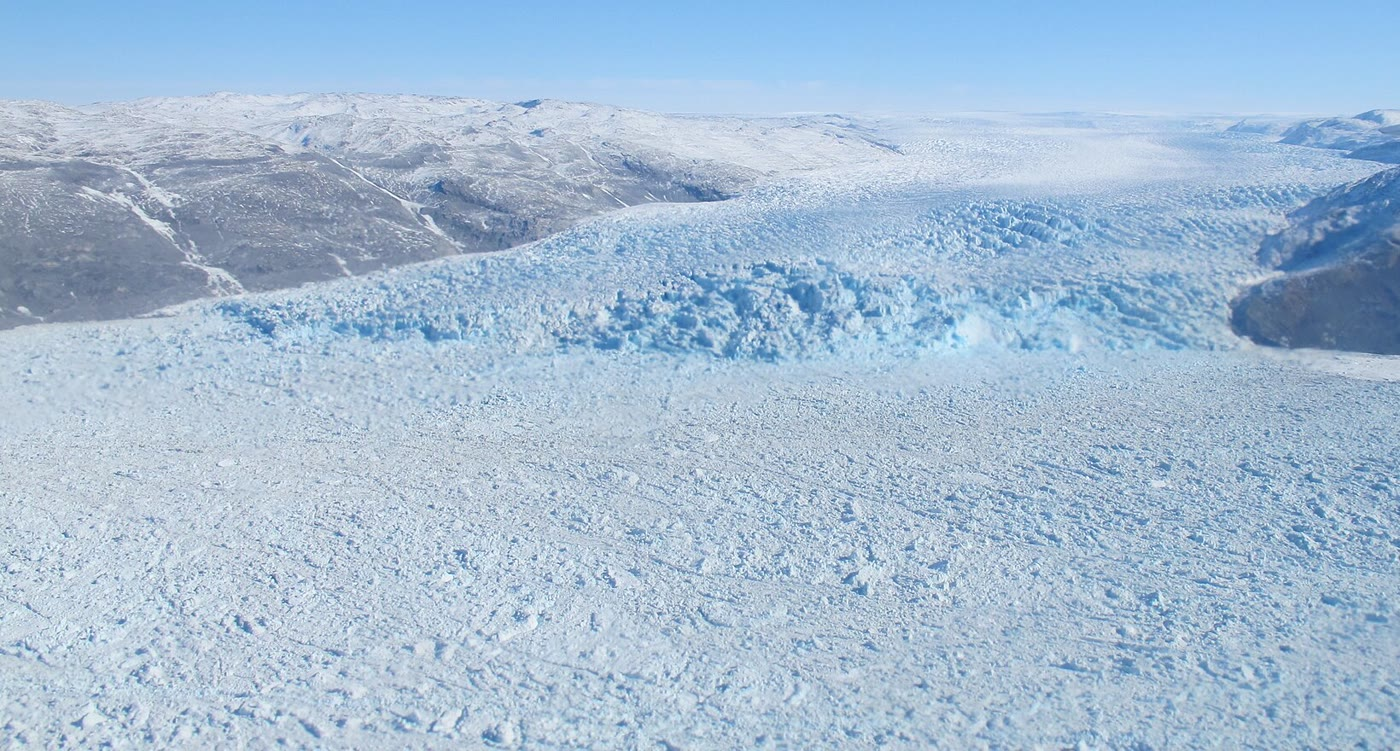
\includegraphics[width=0.82\linewidth]{images/book5/b3-greenland-outlet.jpg}

\par\smallskip{\small Gletser keluaran dari lembaran es Greenland,
di antara pegunungan, berakhir di laut pada front \omterm{def:b3:glaciology:grounding-line}{pelepasan bongkah esnya}, dinding patah
dari es biru yang membentang di tengah gambar; fyord di depannya dipenuhi
dengan bongkah es hasil pelepasan dan es laut. Difoto dari pesawat
Operation IceBridge milik NASA pada April 2014 (NASA / Jim Yungel, domain
publik).}\label{fig:b3:glaciology:outlet}
\end{omfigure}
% ledger: photo:b3-greenland-outlet

\begin{inthefield}[Sebuah kemah di atas es]
\begin{minipage}[t]{0.55\linewidth}\vspace{0pt}
Di atas lembaran es, instrumen para glasiolog dibawa dengan kereta luncur dan
mereka tinggal di dalam tenda. Untuk mengukur seberapa cepat es bergerak, mereka
membenamkan tiang ke dalam salju dan memasang pada tiang itu antena penerima navigasi satelit. Penerima
yang dipakai dalam geodesi menetapkan posisi hingga beberapa sentimeter, sehingga
posisi yang diulang selama beberapa minggu atau musim memberikan laju dan arah
gerak es, dan tinggi tiang yang disurvei ulang memberikan penipisan atau
penebalan es di bawahnya.
\end{minipage}\hfill
\begin{minipage}[t]{0.42\linewidth}\vspace{0pt}
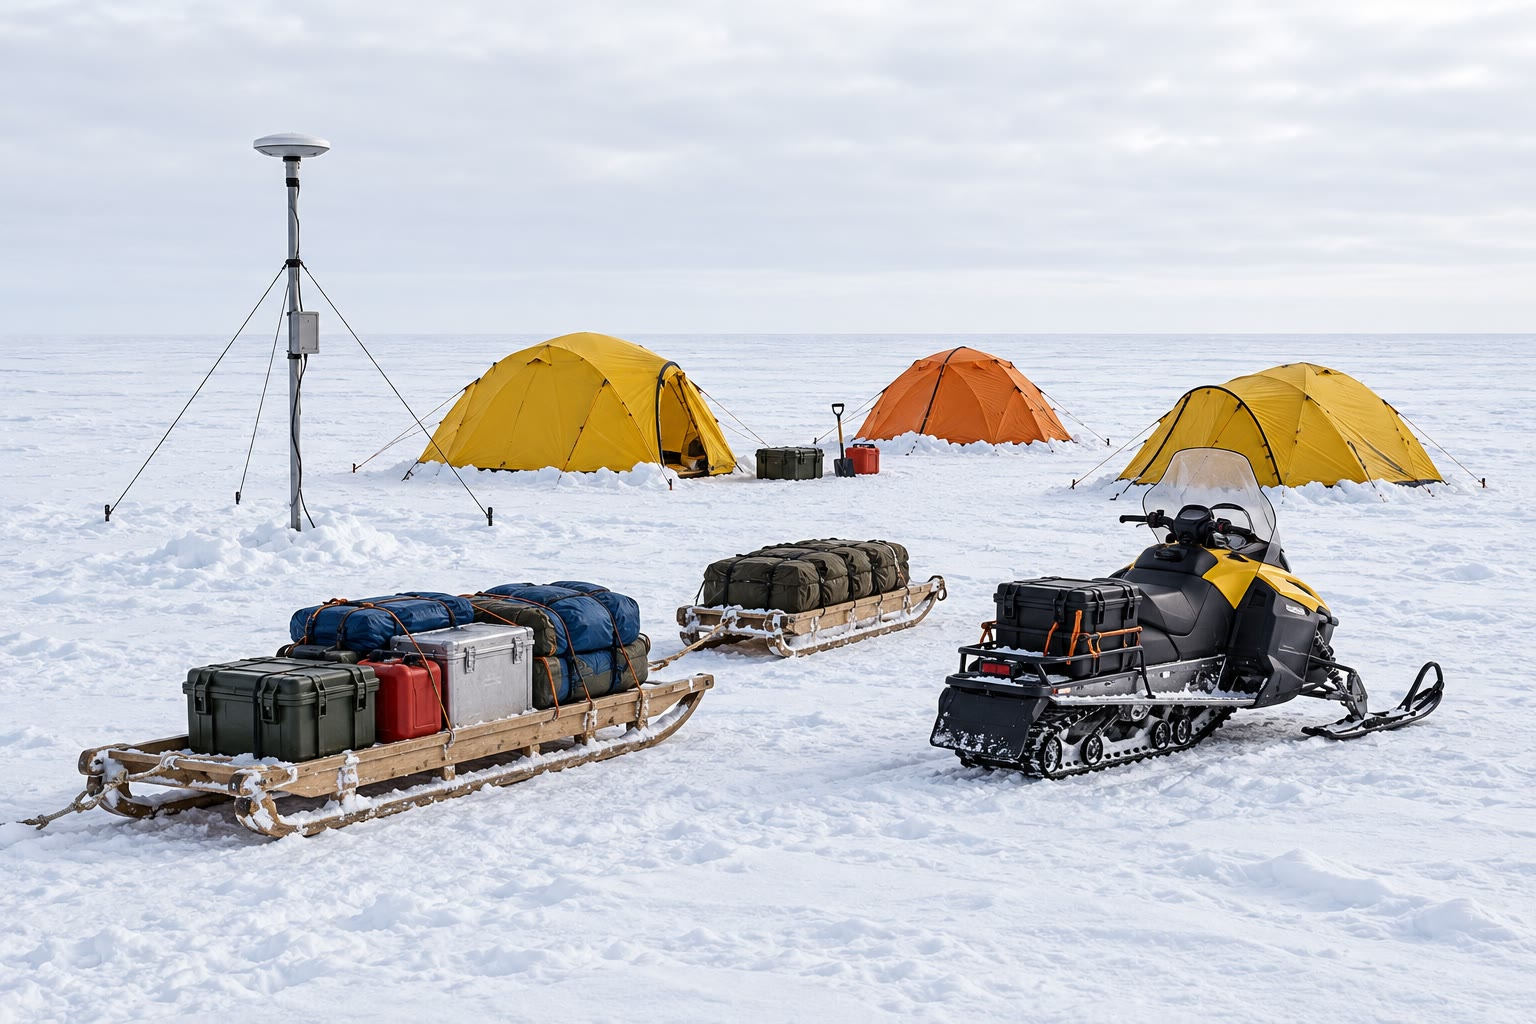
\includegraphics[width=\linewidth]{images/book5/ai/b3-glaciology-camp.jpg}

{\scriptsize Sebuah kemah lapangan di atas lembaran es: tenda, kereta luncur dan
kendaraan salju, serta antena navigasi satelit pada tiang yang ditahan
tali penahan (ilustrasi buatan AI).}
\end{minipage}
\end{inthefield}
% ledger: gps:high-end

\section{Es laut dan permafrost}\label{sec:b3:glaciology:sea-ice}

Es laut terbentuk, bertambah, dan mencair di samudra. Di Arktik, luasnya
mencapai puncak pada Maret dan paling kecil pada September.
% ledger: nsidc:sea-ice-def

\begin{definition}[Luasan es laut]\label{def:b3:glaciology:sea-ice}
Yang disebut \emph{luasan es laut}\index{luasan es laut} adalah total luas dari
sel-sel peta satelit tempat es laut menutupi lebih dari
\qty{15}{\percent} permukaannya. Angka ini lebih besar daripada luas es laut,
yang hanya menghitung es itu sendiri.
\end{definition}
% ledger: nsidc:sea-ice-def

Sejak satelit mulai memetakannya pada 1979, luasan Arktik menyusut, pada
Maret dan jauh lebih besar pada September: sebesar \qty{0.74}{\mega km^2} per dekade
pada September, sekitar \qty{12}{\percent} dari rata-rata 1981--2010 per dekade, dibandingkan
dengan \qty{0.38}{\mega km^2}, \qty{2.5}{\percent}, pada Maret. Luasan September
terkecil sejauh ini, \qty{3.57}{\mega km^2}, terjadi pada 2012. Es laut Arktik
memantulkan \qtyrange{50}{70}{\percent} sinar matahari, sedangkan samudra terbuka
sekitar \qty{6}{\percent}: kehilangan es membuat permukaan lebih gelap, yaitu
umpan balik es--albedo dari volume Tahun~2.
% ledger: data:b5-nsidc-extent, nsidc:sea-ice-reflect

Es laut tumbuh di bagian bawahnya, tempat air laut membeku di atasnya, dan kalor
laten dari pembekuan itu harus dialirkan naik melalui es menuju udara dingin.

\begin{theorem}[Hukum Stefan]\label{thm:b3:glaciology:stefan}
Es laut dengan konduktivitas termal $k_i$, massa jenis $\rho_i$ dan kalor laten
peleburan $L$, dengan permukaannya dipertahankan pada suhu $\Delta T$ di bawah
titik beku air di bawahnya, tumbuh, jika panas dari samudra
dapat diabaikan, sebagai
\[
h(t)^2 - h(0)^2 = \frac{2k_i\,\Delta T}{\rho_iL}\,t .
\]
Di bawah lapisan salju dengan tebal $h_s$ dan konduktivitas $k_s$, laju
pertumbuhannya adalah $\mathrm dh/\mathrm dt = \Delta T/[\rho_iL(h/k_i + h_s/k_s)]$.
\end{theorem}

\begin{proof}
Suhu di dalam es tipis bersifat linear, dari titik beku di dasar
hingga suhu permukaan di puncak, sehingga fluks panas yang melewatinya adalah
$k_i\Delta T/h$, atau, melalui es dan salju yang tersusun seri, $\Delta T/(h/k_i +
h_s/k_s)$. Pembekuan lapisan setebal $\mathrm dh$ melepaskan $\rho_iL\,\mathrm dh$ per
satuan luas, yang harus dibawa pergi oleh fluks ini: $\rho_iL\,\mathrm dh/\mathrm dt
= k_i\Delta T/h$. Maka $\mathrm d(h^2)/\mathrm dt = 2k_i\Delta T/(\rho_iL)$.
\end{proof}

Dengan $k_i = \qty{2.03}{W.m^{-1}.K^{-1}}$, $L = \qty{3.34e5}{J/kg}$ dan
$\rho_i = \qty{917}{kg/m^3}$, permukaan \qty{20}{K} di bawah titik beku
menumbuhkan es setebal \qty{1.5}{m} dalam seratus hari dan \qty{2.1}{m} dalam dua ratus hari.
Salju, dengan konduktivitas \qty{0.30}{W.m^{-1}.K^{-1}}, adalah isolator yang
baik: lapisan \qty{20}{cm} saja memperlambat pertumbuhan lebih dari separuh. Es tebal tumbuh
lambat, es tipis tumbuh cepat: hukum ini cenderung meratakan ketebalan es
setelah satu musim panas lelehan.
% ledger: cice:constants, iapws:ice-density

\begin{omfigure}
\begin{tikzpicture}
\begin{groupplot}[group style={group size=2 by 1, horizontal sep=1.5cm},
  width=0.48\linewidth, height=0.4\linewidth,
  tick label style={font=\scriptsize}, label style={font=\small}, title style={font=\small}]
\nextgroupplot[xlabel={tahun}, ylabel={luasan (\unit{\mega km^2})}, xmin=1977, xmax=2028,
  ymin=0, ymax=18, title={Luasan es laut Arktik},
  xticklabel style={/pgf/number format/1000 sep={}},
  legend style={font=\scriptsize, at={(0.03,0.66)}, anchor=west}]
% computed in figdata/bachelor-3/sea_ice.py
\addplot[omDef, thick, mark=*, mark size=0.9pt] table[x=year, y=mar] {figdata/out/bachelor-3-sea_ice-extent.dat};
\addlegendentry{Maret}
\addplot[omThm, thick, mark=*, mark size=0.9pt] table[x=year, y=sep] {figdata/out/bachelor-3-sea_ice-extent.dat};
\addlegendentry{September}
\addplot[black!60, densely dashed, forget plot] table[x=year, y=mar] {figdata/out/bachelor-3-sea_ice-trend.dat};
\addplot[black!60, densely dashed, forget plot] table[x=year, y=sep] {figdata/out/bachelor-3-sea_ice-trend.dat};
\nextgroupplot[xlabel={hari pembekuan}, ylabel={ketebalan es (\unit{m})}, xmin=0, xmax=200,
  ymin=0, ymax=2.4, title={pertumbuhan, $\Delta T = \qty{20}{K}$},
  legend style={font=\scriptsize, at={(0.97,0.03)}, anchor=south east}]
\addplot[omMeth, thick] table[x=day, y=h0] {figdata/out/bachelor-3-sea_ice-stefan.dat};
\addlegendentry{es tanpa salju}
\addplot[omDef, thick, densely dashed] table[x=day, y=hs] {figdata/out/bachelor-3-sea_ice-stefan.dat};
\addlegendentry{di bawah \qty{20}{cm} salju}
\end{groupplot}
\end{tikzpicture}

\par\smallskip{\small Kiri, rata-rata \omterm{def:b3:glaciology:sea-ice}{luasan es laut} Arktik pada Maret dan pada
September, 1979--2026 (Indeks Es Laut NSIDC, versi~4), dengan kuadrat terkecil
tren (putus-putus): \qty{-0.38}{\mega km^2} dan \qty{-0.74}{\mega km^2} per
dekade. Kanan, pertumbuhan es laut akibat konduksi di bawah permukaan yang
\qty{20}{K} di bawah titik beku, tanpa panas samudra: es tanpa salju menurut hukum Stefan,
dan es yang sama di bawah \qty{20}{cm} salju.}\label{fig:b3:glaciology:sea-ice}
\end{omfigure}
% ledger: data:b5-nsidc-extent, cice:constants

Permafrost adalah tanah yang tetap pada atau di bawah \qty{0}{\celsius} selama dua
tahun atau lebih. Permafrost mendasari sekitar seperempat daratan terbuka di Belahan Bumi
Utara.
% ledger: nsidc:permafrost

\begin{definition}[Lapisan aktif]\label{def:b3:glaciology:permafrost}
Yang disebut \emph{lapisan aktif}\index{lapisan aktif} adalah lapisan tanah di atas
permafrost yang mencair setiap musim panas dan membeku lagi setiap musim dingin.
\end{definition}

Ketebalannya ditentukan, seperti pertumbuhan es laut, oleh konduksi panas ke
dalam tanah selama musim lelehan, melawan kalor laten
es tanah itu. Suhu permafrost telah meningkat selama tiga sampai
empat dekade terakhir di seluruh wilayah permafrost (keyakinan tinggi);
permafrost menghangat secara global sebesar \qty{0.29}{\celsius} [\numrange{0.17}{0.41}]
antara 2007 dan 2016 (keyakinan sedang), dan pertambahan ketebalan
\omterm{def:b3:glaciology:permafrost}{lapisan aktif} merupakan fenomena se-Arktik (keyakinan sedang).
Di tempat es di dalamnya mencair, tanah dapat runtuh.
% ledger: ar6ch9:permafrost, nsidc:permafrost-thaw

\section{Kriosfer dan permukaan laut}\label{sec:b3:glaciology:sea-level}

Anggaran permukaan laut dalam volume Tahun~2 menjumlahkan ekspansi samudra yang
menghangat dengan air yang ditambahkan oleh es dan oleh daratan. Dari
kenaikan permukaan laut sebesar \qty{3.69}{mm/yr} yang teramati selama 2006--2018, gletser
menyumbang \qty{0.62}{mm/yr}, Greenland \qty{0.63}{mm/yr}, dan Antartika
\qty{0.37}{mm/yr}: es secara bersama-sama menyumbang lebih besar daripada ekspansi
samudra, \qty{1.39}{mm/yr}.
% ledger: ar6ch9:table95

\begin{dated}{2021}
Greenland kehilangan \qty{4890}{Gt} es selama 1992--2020 [4140 sampai 5640],
setara \qty{13.5}{mm} permukaan laut, dengan laju yang naik dari \qty{39}{Gt/yr} pada
1990-an menjadi \qty{243}{Gt/yr} pada 2010--2019, akibat pengaliran keluar es dan, makin besar,
akibat pencairan di permukaan (keyakinan tinggi). Antartika kehilangan \qty{2670}{Gt}
[1800 sampai 3540], \qty{7.4}{mm}, dengan lajunya naik dari \qty{49}{Gt/yr} pada
1990-an menjadi \qty{148}{Gt/yr} pada 2010--2019; kehilangan itu berasal dari gletser pengalir Antartika Barat,
terutama melalui pencairan paparan es dari bawah (keyakinan
tinggi). Gletser di luar lembaran es kehilangan \qty{6200}{Gt} selama
1993--2019, \qty{17.1}{mm}, lebih banyak pada 2010--2019 daripada dekade mana pun
dalam catatan (keyakinan sangat tinggi). Greenland akan terus kehilangan massa
sepanjang abad ini di bawah semua skenario yang dipertimbangkan (hampir
pasti), dan Antartika juga (mungkin): pada 2100 Greenland mungkin menambah
\qtyrange{0.01}{0.10}{m} pada permukaan laut di bawah skenario emisi rendah
dan \qtyrange{0.09}{0.18}{m} di bawah skenario emisi sangat tinggi, Antartika
\qtyrange{0.03}{0.27}{m} dan \qtyrange{0.03}{0.34}{m}. Samudra Arktik
mungkin akan hampir sepenuhnya bebas es laut, dengan kurang dari
\qty{1}{\mega km^2} tersisa, pada minimum September untuk pertama kalinya
sebelum 2050 di bawah semua skenario yang dipertimbangkan.
\end{dated}
% ledger: ar6ch9:greenland, ar6ch9:antarctica, ar6ch9:glaciers, ar6ch9:ice-sheet-proj, ar6ch9:sea-ice

Kehilangan lembaran es diperoleh seperti yang dijelaskan di Bab~\ref{ch:b3:gravity-geodesy},
diukur dengan altimetri, dengan gravimetri, dan dengan selisih antara salju yang turun
dan es yang mengalir keluar: tiga metode independen yang digabungkan
menjadi satu taksiran.
% ledger: data:b5-imbie

\section{Latihan}

\begin{exercise}[$\star$]\label{exo:b3:glaciology:1}
Sebuah gletser lembah setebal \qty{250}{m} mengalir menuruni lereng \ang{3}. Hitung
tegangan geser basalnya, lalu bandingkan dengan tegangan basal gletser nyata,
yang besarnya sekitar satu bar.
\end{exercise}

\begin{exercise}[$\star$]\label{exo:b3:glaciology:2}
(a)~Lembaran es Greenland menyimpan sekitar \qty{2.9}{\mega km^3} es dengan
massa jenis \qty{917}{kg/m^3}. Hitung massanya serta \omterm{def:b3:glaciology:sle}{setara permukaan laut} pada
\qty{360}{Gt/mm}, lalu bandingkan dengan \qty{7.4}{m} yang biasa dikutip.
(b)~Lakukan hal yang sama untuk Antarktika dengan \qty{30}{\mega km^3}, yang dikutip sekitar
\qty{58}{m}. Mengapa keduanya tampak berbeda sedemikian jauh?
\end{exercise}
% ledger: nsidc:ice-sheets

\begin{exercise}[$\star$]\label{exo:b3:glaciology:3}
Sebuah gletser memiliki \omterm{def:b3:glaciology:mass-balance}{zona akumulasi} seluas \qty{6}{km^2} dengan neraca rata-rata
\qty{+1.2}{m} setara air, dan \omterm{def:b3:glaciology:mass-balance}{zona ablasi} seluas \qty{4}{km^2} dengan
\qty{-2.1}{m}. Hitung neraca bersihnya dalam meter kubik air, neraca spesifik rata-rata,
dan rasio luas \omterm{def:b3:glaciology:mass-balance}{zona akumulasinya}. Apakah gletser ini tumbuh atau
menyusut?
\end{exercise}

\begin{exercise}[$\star$]\label{exo:b3:glaciology:4}
Pada \omterm{def:b3:glaciology:firn}{penutupan pori}, \omterm{def:b3:glaciology:firn}{firn} memiliki massa jenis \qtyrange{820}{830}{kg/m^3}.
Berapa bagian volumenya yang masih berupa ruang pori (es:
\qty{917}{kg/m^3})?
\end{exercise}
% ledger: firn:close-off

\begin{exercise}[$\star\star$]\label{exo:b3:glaciology:5}
Sebuah gletser temperat (es pada \qty{0}{\celsius}, $A =
\qty{1.4e-16}{Pa^{-3}.yr^{-1}}$) setebal \qty{300}{m} di lereng
\ang{3}. Hitung kecepatan permukaannya hanya dari deformasi internal. Dengan
faktor berapa kecepatan itu akan berubah jika tebalnya dua kali lipat? Jika lerengnya
dibuat setengahnya?
\end{exercise}

\begin{exercise}[$\star\star$]\label{exo:b3:glaciology:6}
Dari konstanta Paterson--Budd, hitung \omterm{def:b3:glaciology:glen}{faktor laju} pada
\qty{-25}{\celsius} dan \qty{-10}{\celsius}, serta rasio kecepatan dua
massa es identik pada \qty{0}{\celsius} dan pada \qty{-25}{\celsius}.
\end{exercise}
% ledger: pism:rheology, codata:R

\begin{exercise}[$\star\star$]\label{exo:b3:glaciology:7}
Hitung ketebalan terbesar lembaran es plastis yang berjarak \qty{1000}{km}
dari pusat ke tepinya dengan $\tau_0 = \qty{100}{kPa}$, lalu bandingkan dengan
ketebalan terbesar es Antarktika, hampir \qty{4.9}{km}.
\end{exercise}
% ledger: nsidc:ice-sheets

\begin{exercise}[$\star\star$]\label{exo:b3:glaciology:8}
Sebuah gletser setebal \qty{200}{m} kehilangan \qty{5}{m} es setiap tahun di ujungnya.
Hitung taksiran waktu responsnya. Jika iklim menghangat mendadak lalu tetap
konstan, berapa lama panjang gletser itu terus berubah?
\end{exercise}

\begin{exercise}[$\star\star$]\label{exo:b3:glaciology:9}
(a)~Dengan hukum Stefan untuk $\Delta T = \qty{20}{K}$, hitung ketebalan
es laut tanpa salju setelah 100 hari, dan waktu yang diperlukan untuk mencapai \qty{3}{m}.
(b)~Apa implikasinya bagi es yang lebih tebal dari \qty{3}{m}?
\end{exercise}
% ledger: cice:constants

\begin{exercise}[$\star\star\star$]\label{exo:b3:glaciology:10}
(a)~Jika dasar berada \qty{800}{m} di bawah permukaan laut, berapa tebal es di
\omterm{def:b3:glaciology:grounding-line}{garis kandas}? (b)~Dengan fluks lempengan $q \propto H^{n+2}$ untuk suatu
kemiringan permukaan tertentu, dengan faktor berapa fluks es yang bertumpu di dasar naik jika
\omterm{def:b3:glaciology:grounding-line}{garis kandas} mundur ke tempat dasar berada \qty{900}{m} di bawah permukaan? (c)~Jelaskan
mengapa dasar yang menurun ke arah daratan membuat mundurnya garis itu saling memperkuat, dan
apa yang diubah oleh paparan es.
\end{exercise}
% ledger: iapws:ice-density, noaa:seawater-1025

\begin{exercise}[$\star\star\star$]\label{exo:b3:glaciology:11}
Tunjukkan bahwa volume tudung es plastis berbentuk lingkaran berjari-jari $R$ adalah $V =
\frac{8\pi}{15}\sqrt{2\tau_0/(\rho g)}\,R^{5/2}$. Dengan faktor berapa
\omterm{def:b3:glaciology:sle}{setara permukaan lautnya} membesar jika jari-jarinya menjadi dua kali lipat?
\end{exercise}

\begin{exercise}[$\star\star\star$]\label{exo:b3:glaciology:12}
Luasan rata-rata es laut Arktik adalah \qty{16.34}{\mega km^2} pada Maret 1979 dan
\qty{14.13}{\mega km^2} pada Maret 2026; pada September, \num{7.05} dan
\qty{4.81}{\mega km^2}. (a)~Hitung perubahan relatif pada setiap bulan.
(b)~Berikan dua alasan fisis mengapa luasan pada September turun
jauh lebih cepat daripada luasan pada Maret.
\end{exercise}
% ledger: data:b5-nsidc-extent

\section{Soal: Tudung es Arkel}

\begin{problem}[{Soal akhir pekan --- bentuk, aliran, neraca, dan
setara permukaan laut tudung es rekaan}]
\label{pb:b3:glaciology:1}
Tudung es rekaan Arkel terletak di atas dataran tinggi datar. Bentuknya hampir bundar,
berjari-jari \qty{20}{km}, dan esnya bersuhu sekitar \qty{-10}{\celsius}. Ambil
$\rho = \qty{917}{kg/m^3}$ dan $g = \qty{9.81}{m/s^2}$.

\medskip\noindent\textbf{Bagian I --- Apakah tudung es ini plastis?}
\begin{enumerate}
\item Tunjukkan bahwa di bawah es setebal $H$ dengan kemiringan permukaan yang kecil
  $\alpha$, tegangan geser basal kira-kira $\rho gH\alpha$.
\item Sondase radar dan survei pada jarak 5, 10, dan \qty{15}{km} dari pusat
  memberikan ketebalan 580, 470, dan \qty{335}{m} serta kemiringan permukaan sebesar
  \num{0.0190}, \num{0.0240}, dan \num{0.0330}. Hitung tegangan geser basal
  di ketiga titik tersebut.
\item Apakah tudung es ini mendekati plastis? Tegangan luluh berapa yang kamu pilih?
\item Dengan $\tau_0 = \qty{100}{kPa}$, hitung $2\tau_0/(\rho g)$.
\item Perkirakan ketebalan di ketiga titik dari profil plastis
  lalu bandingkan dengan sondase.
\end{enumerate}

\medskip\noindent\textbf{Bagian II --- Bentuk dan volume.}
\begin{enumerate}[resume]
\item Hitung ketebalan di pusat.
\item Tunjukkan bahwa volumenya adalah $V = \frac{8\pi}{15}\sqrt{2\tau_0/(\rho
  g)}\,R^{5/2}$.
\item Hitung volume dalam kilometer kubik.
\item Hitung luas dan ketebalan rata-rata.
\item Tudung es yang dua kali lebih lebar di dataran tinggi yang sama: dengan faktor berapa
  volumenya lebih besar?
\end{enumerate}

\medskip\noindent\textbf{Bagian III --- Aliran dan neraca.}
\begin{enumerate}[resume]
\item Hitung \omterm{def:b3:glaciology:glen}{faktor laju} pada \qty{-10}{\celsius} dalam
  \unit{Pa^{-3}.yr^{-1}}.
\item Pada jarak \qty{10}{km} dari pusat, dengan memperlakukan es sebagai lempengan,
  hitung kelajuan permukaan akibat deformasi internal.
\item Hitung fluks es per satuan lebar di sana, dan kelajuan rata-rata
  kolom tersebut.
\item Dalam keadaan tunak, fluks yang meninggalkan lingkaran berjari-jari
  \qty{10}{km} sama dengan neraca yang diperoleh di dalamnya. Berapa neraca rata-rata, dalam
  meter es per tahun, yang diperlukan untuk hal ini?
\item Garis kesetimbangan terletak \qty{450}{m} di atas dataran tinggi. Di mana letaknya
  pada tudung es, dan berapa rasio luas akumulasi?
\item Jika es menghangat hingga \qty{0}{\celsius}, berapa kali lipat
  kelajuannya akan naik? Apa yang akan terjadi pada bentuk tudung es?
\end{enumerate}

\medskip\noindent\textbf{Bagian IV --- Permukaan laut.}
\begin{enumerate}[resume]
\item Hitung massa tudung es dalam gigaton.
\item Hitung \omterm{def:b3:glaciology:sle}{setara permukaan laut} dalam milimeter.
\item Jika seluruh tudung menipis \qty{0.5}{m} es per tahun tanpa mengalir,
  berapa lama tudung itu akan bertahan?
\item Mengapa tudung es sungguhan akan lenyap lebih cepat dari itu, begitu
  mulai menipis?
\item Dengan laju hilangnya es Greenland pada 2010--2019, berapa lama
  waktu yang diperlukan untuk kehilangan massa yang sama dengan tudung es Arkel?
\item Berikan \omterm{def:b3:glaciology:sle}{setara permukaan laut} dari tudung es Arkel, dalam milimeter,
  dengan satu angka desimal.
\end{enumerate}
\end{problem}
% ledger: pism:rheology, data:b5-imbie, ar6ch9:greenland, ar6ch9:faq91
